\documentclass[12pt,a4paper]{article}

\usepackage[in, plain]{fullpage}
\usepackage{array}
%\usepackage{../../../pas-math}
\usepackage{../../../moncours2}


%\usepackage{pas-cours}
%%-------------------------------------------------------------------------------
%          -Packages nécessaires pour écrire en Français et en UTF8-
%-------------------------------------------------------------------------------
\usepackage[utf8]{inputenc}
\usepackage[frenchb]{babel}
\usepackage[T1]{fontenc}
\usepackage{lmodern}
\usepackage{textcomp}



%-------------------------------------------------------------------------------

%-------------------------------------------------------------------------------
%                          -Outils de mise en forme-
%-------------------------------------------------------------------------------
\usepackage{hyperref}
\hypersetup{pdfstartview=XYZ}
%\usepackage{enumerate}
\usepackage{graphicx}
\usepackage{multicol}
\usepackage{tabularx}
\usepackage{multirow}


\usepackage{anysize} %%pour pouvoir mettre les marges qu'on veut
%\marginsize{2.5cm}{2.5cm}{2.5cm}{2.5cm}

\usepackage{indentfirst} %%pour que les premier paragraphes soient aussi indentés
\usepackage{verbatim}
\usepackage{enumitem}
\usepackage[usenames,dvipsnames,svgnames,table]{xcolor}

\usepackage{variations}

%-------------------------------------------------------------------------------


%-------------------------------------------------------------------------------
%                  -Nécessaires pour écrire des mathématiques-
%-------------------------------------------------------------------------------
\usepackage{amsfonts}
\usepackage{amssymb}
\usepackage{amsmath}
\usepackage{amsthm}
\usepackage{tikz}
\usepackage{xlop}
%-------------------------------------------------------------------------------



%-------------------------------------------------------------------------------


%-------------------------------------------------------------------------------
%                    - Mise en forme avancée
%-------------------------------------------------------------------------------

\usepackage{ifthen}
\usepackage{ifmtarg}


\newcommand{\ifTrue}[2]{\ifthenelse{\equal{#1}{true}}{#2}{$\qquad \qquad$}}

%-------------------------------------------------------------------------------

%-------------------------------------------------------------------------------
%                     -Mise en forme d'exercices-
%-------------------------------------------------------------------------------
%\newtheoremstyle{exostyle}
%{\topsep}% espace avant
%{\topsep}% espace apres
%{}% Police utilisee par le style de thm
%{}% Indentation (vide = aucune, \parindent = indentation paragraphe)
%{\bfseries}% Police du titre de thm
%{.}% Signe de ponctuation apres le titre du thm
%{ }% Espace apres le titre du thm (\newline = linebreak)
%{\thmname{#1}\thmnumber{ #2}\thmnote{. \normalfont{\textit{#3}}}}% composants du titre du thm : \thmname = nom du thm, \thmnumber = numéro du thm, \thmnote = sous-titre du thm

%\theoremstyle{exostyle}
%\newtheorem{exercice}{Exercice}
%
%\newenvironment{questions}{
%\begin{enumerate}[\hspace{12pt}\bfseries\itshape a.]}{\end{enumerate}
%} %mettre un 1 à la place du a si on veut des numéros au lieu de lettres pour les questions 
%-------------------------------------------------------------------------------

%-------------------------------------------------------------------------------
%                    - Mise en forme de tableaux -
%-------------------------------------------------------------------------------

\renewcommand{\arraystretch}{1.7}

\setlength{\tabcolsep}{1.2cm}

%-------------------------------------------------------------------------------



%-------------------------------------------------------------------------------
%                    - Racourcis d'écriture -
%-------------------------------------------------------------------------------

% Angles orientés (couples de vecteurs)
\newcommand{\aopp}[2]{(\vec{#1}, \vec{#2})} %Les deuc vecteurs sont positifs
\newcommand{\aopn}[2]{(\vec{#1}, -\vec{#2})} %Le second vecteur est négatif
\newcommand{\aonp}[2]{(-\vec{#1}, \vec{#2})} %Le premier vecteur est négatif
\newcommand{\aonn}[2]{(-\vec{#1}, -\vec{#2})} %Les deux vecteurs sont négatifs

%Ensembles mathématiques
\newcommand{\naturels}{\mathbb{N}} %Nombres naturels
\newcommand{\relatifs}{\mathbb{Z}} %Nombres relatifs
\newcommand{\rationnels}{\mathbb{Q}} %Nombres rationnels
\newcommand{\reels}{\mathbb{R}} %Nombres réels
\newcommand{\complexes}{\mathbb{C}} %Nombres complexes


%Intégration des parenthèses aux cosinus
\newcommand{\cosP}[1]{\cos\left(#1\right)}
\newcommand{\sinP}[1]{\sin\left(#1\right)}


%Probas stats
\newcommand{\stat}{statistique}
\newcommand{\stats}{statistiques}
%-------------------------------------------------------------------------------

%-------------------------------------------------------------------------------
%                    - Mise en page -
%-------------------------------------------------------------------------------

\newcommand{\twoCol}[1]{\begin{multicols}{2}#1\end{multicols}}


\setenumerate[1]{font=\bfseries,label=\textit{\alph*})}
\setenumerate[2]{font=\bfseries,label=\arabic*)}


%-------------------------------------------------------------------------------
%                    - Elements cours -
%-------------------------------------------------------------------------------





%\makeatletter
%\renewcommand*{\@seccntformat}[1]{\csname the#1\endcsname\hspace{0.1cm}}
%\makeatother


%\toggletrue{eleve}
%\toggletrue{dys}



%\author{Olivier FINOT}
\date{}
\title{\textcircled{{\normalsize{1}}} Nombres entiers et décimaux}
%\title{\tikz \node[draw,circle]{1}; Nombres entiers et décimaux}
\lhead{CH1 : Nombres entiers et décimaux}
\rhead{O. FINOT}
%
%\rfoot{Page \thepage}
\begin{document}
\maketitle

\setenumerate[1]{label=\textbf{\arabic*)}}

%\chap[num=1, color=red]{Nombres entiers et décimaux}{Olivier FINOT, \today }

\begin{myobj}
	\begin{itemize}
		
		\item Construire le symétrique d’un point ou d'une figure par rapport à une droite à la main où à l’aide d’un logiciel;
		\item Construire le symétrique d’un point ou d'une figure par rapport à un point, à la main où à l’aide d’un logiciel;
		\item Utiliser les propriétés de la symétrie axiale ou centrale;
		\item Identifier des symétries dans des figures.		
	\end{itemize}
\end{myobj}

\begin{mycomp}
	\begin{itemize}
		\item \kw{Chercher (Ch2)} :  s’engager    dans    une    démarche    scientifique, observer, questionner, manipuler, expérimenter (sur une feuille de papier, avec des objets, à l’aide de logiciels), émettre des hypothèses, chercher des exemples ou des contre-exemples, simplifier ou particulariser une situation, émettre une conjecture ;
		\item \kw{Raisonner (Ra3)} :  démontrer : utiliser un raisonnement logique et des règles établies (propriétés, théorèmes, formules) pour parvenir à une conclusion ;
		\item \kw{Communiquer (Co2)} :  expliquer à l’oral ou à l’écrit (sa démarche, son raisonnement, un calcul, un protocole   de   construction   géométrique, un algorithme), comprendre les explications d’un autre et argumenter dans l’échange ; 
		
	\end{itemize}
\end{mycomp}




\vspace*{-0.5cm}

\section{\'Ecrire un nombre}\label{sec:ecrire-un-nombre}

%\begin{myact}{1 Différentes écritures des nombres}
%
%	\label{act:nbres}
%	
%	\begin{enumerate}
%		\item Donner deux nombres à 2, 3, 4 et 5 chiffres.
%		
%		%\item \'Ecrire les nombres suivants en toutes lettres : \num{32}, \num{128} et \num{1024}. 
%		\item \'Ecrire  le nombre 25146041337 en séparant les classes.
%		\item La planète Mars a un rayon d'environ \textbf{3,4 milliers} de km, une superficie d'environ \textbf{144,8 millions} de $km^2$ et un volume d'environ \textbf{163 milliards} de $km^3$.
%		
%		\'Ecrire les trois nombres en gras en utilisant que des chiffres.
%		
%		\item Lire le texte ci-dessous, puis écrire en chiffres les nombres en gras.
%		
%			\begin{center}
%				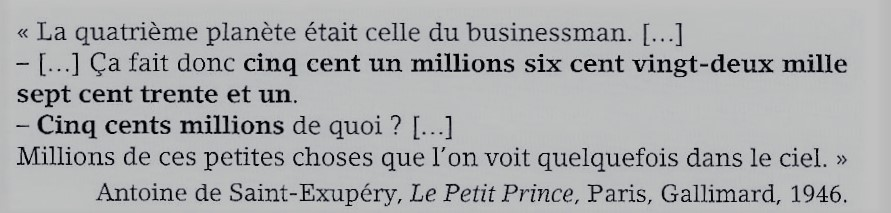
\includegraphics[scale=1.1]{img/act1}
%			\end{center}
%	\end{enumerate}
%\end{myact}

%\begin{myactrep}{1 Différentes écritures des nombres}
	
%	\begin{enumerate}
%		\item 
%			\begin{itemize}
%				\item 17 et 42 sont des nombres à 2 chiffres;
%				\item 128 et 512 sont des nombres à 3 chiffres;
%				\item \num{2048} et \num{4096} sont des nombres à 4 chiffres;
%				\item \num{16384} et \num{65536} sont des nombres à 5 chiffres.
%			\end{itemize}
%		
%		%\item \'Ecrire les nombres suivants en toutes lettres : \num{32}, \num{128} et \num{1024}. 
%		\item Le nombre 25146041337 s'écrit \num{25146041337}.
%		\item 
%			\begin{itemize}
%				\item 3,4 milliers s'écrit \num{3400};
%				\item 144,8 millions s'écrit \num{144800000};
%				\item 163 milliards s'écrit \num{163000000000}.
%			\end{itemize}
%		
%		\item .
%			\begin{itemize}
%				\item Cinq-cent-un-millions-six-cent-vingt-deux-mille-sept-cent trente-et-un s'écrit \num{501622731};
%				\item Cinq-cent-millions s'écrit \num{500000000}.
%			\end{itemize}
%
%	\end{enumerate}
%\end{myactrep}


\begin{mydef}
	\begin{itemize}
		\item Il existe 10 \kw{chiffres} : 
		\iftoggle{eleve}{%
			\iftoggle{dys}{%
				0, 1, 2, 3, 4, 5, 6, 7, 8 et 9.	
			}{
		}
		}{%
			0, 1, 2, 3, 4, 5, 6, 7, 8 et 9.	
		}
		
		\item On utilise les chiffres pour  
		\iftoggle{eleve}{%
			\iftoggle{dys}{%
				écrire des	nombres
			}{
			}
		}{%
			écrire des nombres
		}.
		
		
	\end{itemize}
\end{mydef}

\begin{myexs}
	\begin{enumerate}
		\item Quels nombres peut-on écrire avec les chiffres  2 et 4 ?
		
		\iftoggle{eleve}{%
			\iftoggle{dys}{%
				On peut écrire les nombres 
			}{
				\vspace*{0.5cm}
			}
		}{%
			On peut écrire les nombres 24 et 42.
		}
		
		\item Le nombre \num{49096} s'écrit avec quels chiffres ? 
		
		\iftoggle{eleve}{%
			\iftoggle{dys}{%
				Il s'écrit avec les chiffres 4, 0, 9 et 6.
			}{
				\vspace*{0.5cm}
			}
		}{%
			Il s'écrit avec les chiffres 4, 0, 9 et 6.
		}
		
		
	\end{enumerate}
\end{myexs}





\begin{mydefs}
	\begin{itemize}
		\item Pour mieux lire un grand nombre, on regroupe \iftoggle{eleve}{%
			\iftoggle{dys}{%
				 ses chiffres en classes par groupe de 3.
			}{
				\vspace*{0.75cm}
			}
		}{%
			 ses chiffres en classes par groupe de 3.
		}
		
		\item Un \kw{nombre décimal} possède \iftoggle{eleve}{%
			\iftoggle{dys}{%
				une \kw{partie entière} (avant la virgule) et une \kw{partie décimale} (après la virgule).
			}{
				\vspace*{0.75cm}
			}
		}{%
			une \kw{partie entière} (avant la virgule) et une \kw{partie décimale} (après la virgule).
		}
		
		\item Un \kw{nombre entier} est un nombre décimal où 
		\iftoggle{eleve}{%
			\iftoggle{dys}{%
				 la partie décimale ne contient que des zéros. Dans ce cas la partie décimale n'apparait pas.
			}{
				\vspace*{0.75cm}\\
				Dans ce cas la partie décimale n'apparait pas.
			}
		}{%
			 la partie décimale ne contient que des zéros. Dans ce cas la partie décimale n'apparait pas.
		} 
		
	\end{itemize}
\end{mydefs}

\begin{center}
	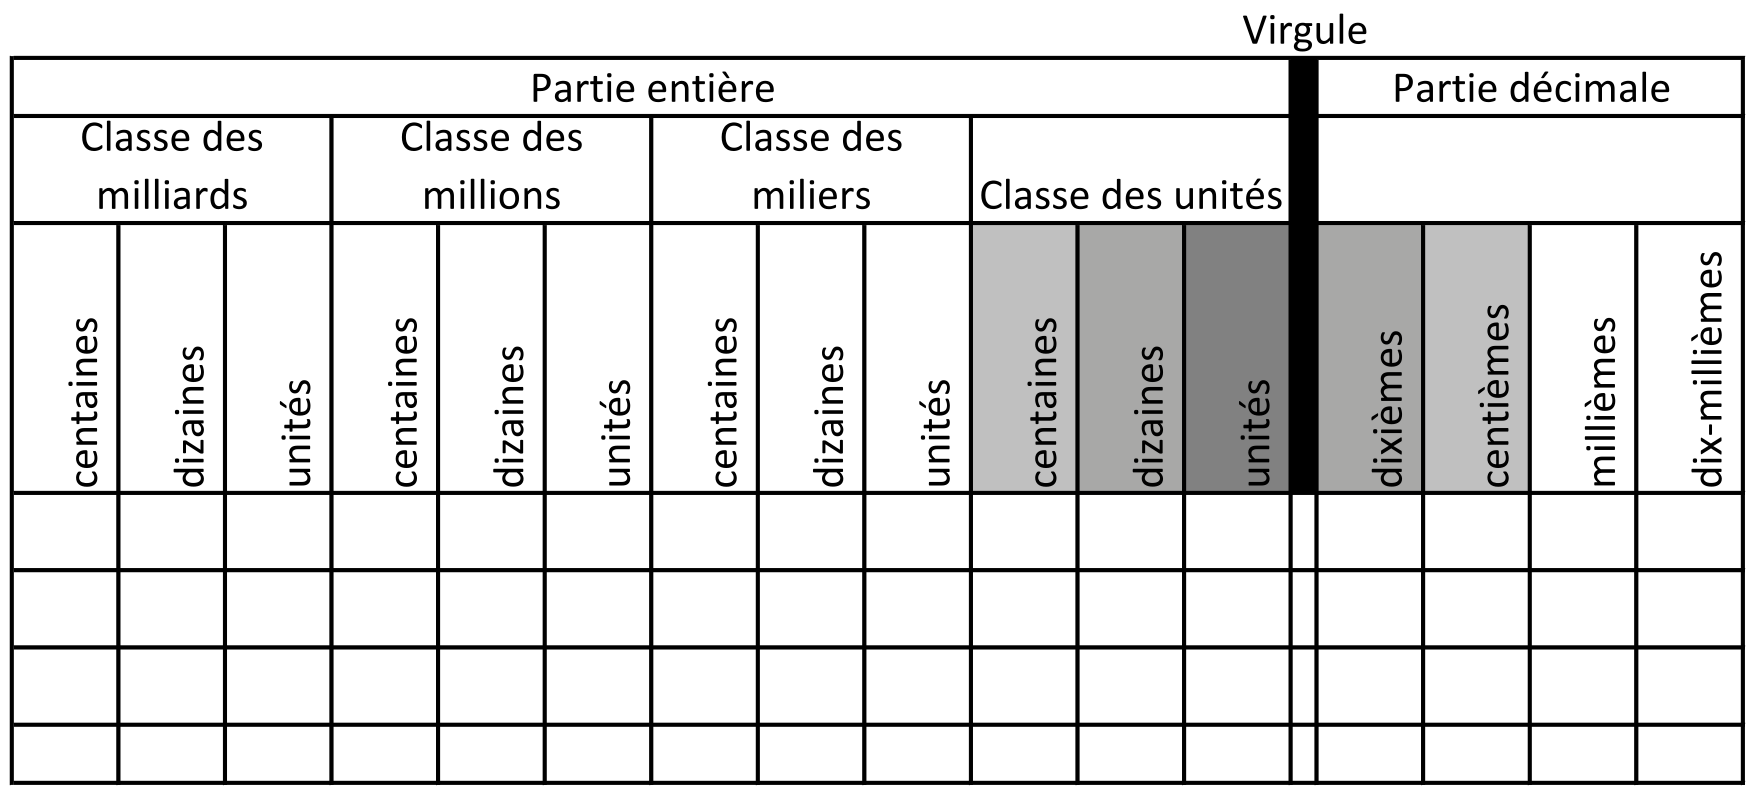
\includegraphics[scale=0.34]{img/tab_rangs}
\end{center}

\begin{myexs}
	\begin{enumerate}
		\item \'Ecrire correctement le nombre 1845937126 :
		
		\iftoggle{eleve}{%
			\iftoggle{dys}{%
				Ce nombre s'écrit 
			}{
				\vspace*{1cm} %\ \\
				
			}
		}{%
			Ce nombre s'écrit \num{1845937126}.
		} 
		
		%\item Le nombre \num{2048} est un nombre entier.
		\item Donner la partie entière et la partie décimale de  \num{5239.67} :
		
		\iftoggle{eleve}{%
			\iftoggle{dys}{%
				La partie entière de   \num{5239.67} est \hspace*{3cm} et sa partie décimale est 	
			}{
				\vspace*{1cm} %\ \\
				
			}
		}{%
			La partie entière de   \num{5239.67} est \num{5239} et sa partie décimale est 67.	
		}
	
		
		
		
		
		\item Donner le chiffre des centaines et le nombre de dizaines de \num{1337}.
		
		
		\iftoggle{eleve}{%
			\iftoggle{dys}{%
				Dans \num{1337}, le chiffre des centaines est \hspace*{2cm} et le nombre de dizaines est \hspace*{2cm}.
			}{
				\vspace*{1cm} %\ \\
				
			}
		}{%
			Dans \num{1337}, le chiffre des centaines est 3 et le nombre de dizaines est 133.
		}
		
		
		\item Donner une autre écriture possible du nombre 124 :
		
		\iftoggle{eleve}{%
			\iftoggle{dys}{%
				Le nombre entier \num{124} peut aussi s'écrire 
			}{
				\vspace*{1cm} %\ \\
				
			}
		}{%
			Le nombre entier \num{124} peut aussi s'écrire \num{124.00}.
		}
	

	\end{enumerate}
\end{myexs}


\begin{mymethname}{\'Ecrire un nombre en toutes lettres}
	\begin{itemize}
		\item Tous les mots qui désignent un nombre sont invariables, sauf <<vingt>> et <<cent>>;
		\item Les mots <<milliard>>, <<million>>, <<dixième>> ne désignent pas des nombres, ils prennent un <<s>> au pluriel;
		\item 80 s'écrit <<quatre-vingts>> sauf s'il est suivi d'un autre nombre;
		\item 100 s'écrit <<cents>> s'il est multiplié et non suivi d'un autre nombre, dans les autres cas il ne prend pas de <<s>>;
		\item On écrit un trait d'union entre chaque mot d'un nombre.
	\end{itemize}
\end{mymethname}

\begin{myexs}
	
	\iftoggle{eleve}{%
		\begin{itemize}
			\item 180 s'écrit %\pause <<cent-quatre-vingts>>;\pause
			\item \num{1300} s'écrit %\pause <<mille-trois-cents>>;\pause
			\item \num{4025035} s'écrit %\pause <<quatre-millions-vingt-cinq-mille-trente-cinq>>;
			\item \num{134.25} s'écrit %\pause <<cent-trente-quatre unités vingt-cinq centièmes.
		\end{itemize}
	}{%
		\begin{itemize}
			\item 180 s'écrit \pause <<cent-quatre-vingts>>;\pause
			\item \num{1300} s'écrit \pause <<mille-trois-cents>>;\pause
			\item \num{4025035} s'écrit \pause <<quatre-millions-vingt-cinq-mille-trente-cinq>>;
			\item \num{134.25} s'écrit \pause <<cent-trente-quatre unités vingt-cinq centièmes.
		\end{itemize}
	}
	
\end{myexs}

%\begin{myexos}
%	\begin{itemize}
%		\item Exercices 1 et 2 page 16 : identifier les chiffres d'un rang donné;
%		\item \Exo{4}{16} : décomposition d'un nombre;
%		\item \Exo{7}{16} : \'ecriture décimale d'un nombre donné en toutes lettres;
%		\item Exercices 8 ,9 et 13 page 17 : problèmes identifier des nombres selon des critères donnés.
%		\item \Exo{11}{17} : regroupement des chiffres d'un nombre en classes.
%		\item \Exo{14}{17} : enlever les zéros inutiles.
%	\end{itemize}
%	
%\end{myexos}


%\newpage

%\section{Multiplier et diviser par 10, 100, 1000}
%
%
\subsection{Multiplier}

\begin{mymeth}
	Pour multiplier un nombre par 10, 100 ou 1000 :
	\begin{enumerate}
		\item on repère la virgule;
		\item on la décale vers la droite d'un rang ($\times 10$) , de deux rangs ($\times 10$) ou de trois ($\times 10$);
		\item on rajoute des zéros si besoin entre le chiffre le plus à droite et la virgule.
	\end{enumerate}
\end{mymeth}

	\begin{myexs}
		\begin{multicols}{2}
			\begin{itemize}
				\item $\num{25.26} \times 10 = \num{252.6}$ 
				\item $\num{25.26} \times 100 = \num{2526.0} = \num{24526}$
				%\item $\num{245.26} \times 1000 = \num{245260}$
				\item $\num{285} \times 10 = \num{285.0} \times \num{10}= \num{2850}$ 
				\item $\num{285} \times 1000 = \num{285000}$ 
			\end{itemize}	
		\end{multicols}
		
	\end{myexs}


\subsection{Diviser}

	\begin{mymeth}
		Pour diviser un nombre par 10, 100 ou 1000 :
		\begin{enumerate}
			\item on repère la virgule;
			\item on la décale vers la gauche d'un rang ($\times 10$) , de deux rangs ($\times 10$) ou de trois ($\times 10$);
			\item on rajoute des zéros si besoin entre la virgule et le chiffre le plus à gauche.
		\end{enumerate}
	\end{mymeth}


	\begin{myexs}
		\begin{multicols}{2}
			\begin{itemize}
				\item $\num{25.26} \div 10 = \num{2.526}$ 
				\item $\num{25.26} \div 1000 = \num{0.02526} $
				%\item $\num{245.26} \times 1000 = \num{245260}$
				\item $\num{285} \div 10 = \num{28.5} $ 
				\item $\num{285} \div 1000 = \num{0.285}$ 
			\end{itemize}	
		\end{multicols}
		
	\end{myexs}

	\begin{myprops}
		\begin{itemize}
			\item Multiplier un nombre par \num{0.1}, \num{0.01} ou \num{0.001} revient à le diviser par 10, 100 ou 1000.
			
			\item A l'inverse, diviser un nombre par \num{0.1}, \num{0.01} ou \num{0.001} revient à le multiplier par 10, 100 ou 1000.
		\end{itemize}
	\end{myprops}

	\begin{myexs}
		%\begin{multicols}{2}
			\begin{itemize}
				\item $\num{45.78} \times \num{0.1} = \num{45.78} \div \num{10} = \num{4.578}$ 
				\item $\num{45.78} \times \num{0.01} = \num{45.78} \div \num{100} = \num{0.4578}$ 
				\item $\num{45.78} \div \num{0.1} = \num{45.78} \times \num{10} = \num{457.8}$ 
				\item $\num{45.78} \div \num{0.001} = \num{45.78} \times \num{1000} = \num{45780}$ 
			\end{itemize}	
		%\end{multicols}
		
	\end{myexs}

	\begin{myexos}
		\begin{itemize}
			\item \Exo{5}{16} : Décomposition d'un nombre et multiplications par dizaines;
			\item \Exo{15}{17} : Nombre d'unités de dizaines etc. complètes
			
		\end{itemize}
	\end{myexos}

\subsection{Fractions décimales}



\begin{myact}{3}
	Activité 2 page 12
\end{myact}


\begin{myactrep}{2 page 12}
	\begin{enumerate}
		\item Je convertis les fractions en nombre décimal :
		
		$ \dfrac{3}{100} = 3 \div 100 = \num{0.03}$ ; $\dfrac{91}{100} = 91 \div 100 = \num{0.91}$; $\dfrac{956}{100} = 956 \div 100 = \num{9.56}$; $\dfrac{18}{1000} = 18 \div 1000 = \num{0.018}$
		
		J'additionne ces nombres aux temps et j'obtiens :
		
		\begin{tabular}{|@{\ }c@{\ }|@{\ }c@{\ }|@{\ }c@{\ }|@{\ }c@{\ }|@{\ }c@{\ }|@{\ }c@{\ }|@{\ }c@{\ }|@{\ }c@{\ }|@{\ }c@{\ }|}
			\hline
			Appel à      & Léa         & Chloé       & Djamila      & Sarah        & Marine      & Sophiane    & Cindy        & Charlotte    \\ \hline
			Temps (en s) & \num{19.98} & \num{20.03} & \num{29.690} & \num{19.893} & \num{19.91} & \num{28.56} & \num{20.018} & \num{19.935} \\ \hline
		\end{tabular}
		
		C'est donc avec Djamila qu'elle a passé le plus de temps et avec Sarah le moins.
		
		\item Je classe les appels téléphoniques du plus court au plus long :
		
		Sarah, Marine, Charlotte, Léa, Cindy, Chloé, Sophiane, Djamila.
	\end{enumerate}
\end{myactrep}



%%
%%
%\section{Fractions décimales}
%%
%



\begin{myact}{3}
	Activité 2 page 12
\end{myact}


\begin{myactrep}{2 page 12}
	\begin{enumerate}
		\item Je convertis les fractions en nombre décimal :
		
		$ \dfrac{3}{100} = 3 \div 100 = \num{0.03}$ ; $\dfrac{91}{100} = 91 \div 100 = \num{0.91}$; $\dfrac{956}{100} = 956 \div 100 = \num{9.56}$; $\dfrac{18}{1000} = 18 \div 1000 = \num{0.018}$
		
		J'additionne ces nombres aux temps et j'obtiens :
		
		\begin{tabular}{|@{\ }c@{\ }|@{\ }c@{\ }|@{\ }c@{\ }|@{\ }c@{\ }|@{\ }c@{\ }|@{\ }c@{\ }|@{\ }c@{\ }|@{\ }c@{\ }|@{\ }c@{\ }|}
			\hline
			Appel à      & Léa         & Chloé       & Djamila      & Sarah        & Marine      & Sophiane    & Cindy        & Charlotte    \\ \hline
			Temps (en s) & \num{19.98} & \num{20.03} & \num{29.690} & \num{19.893} & \num{19.91} & \num{28.56} & \num{20.018} & \num{19.935} \\ \hline
		\end{tabular}
		
		C'est donc avec Djamila qu'elle a passé le plus de temps et avec Sarah le moins.
		
		\item Je classe les appels téléphoniques du plus court au plus long :
		
		Sarah, Marine, Charlotte, Léa, Cindy, Chloé, Sophiane, Djamila.
	\end{enumerate}
\end{myactrep}

\begin{mydef}
	\begin{itemize}
		\item Une \kw{fraction}, notée $\dfrac{n}{d}$ est une division entre deux nombres $n$ et $d$, séparés par un trait de fraction.
		
		\item $n$ est le \kw{numérateur} , $d$ est le \kw{dénominateur}.
	\end{itemize}

	
	
\end{mydef}

\begin{myex}
	$\dfrac{15}{5}$ est une fraction.
	
	\begin{center}
		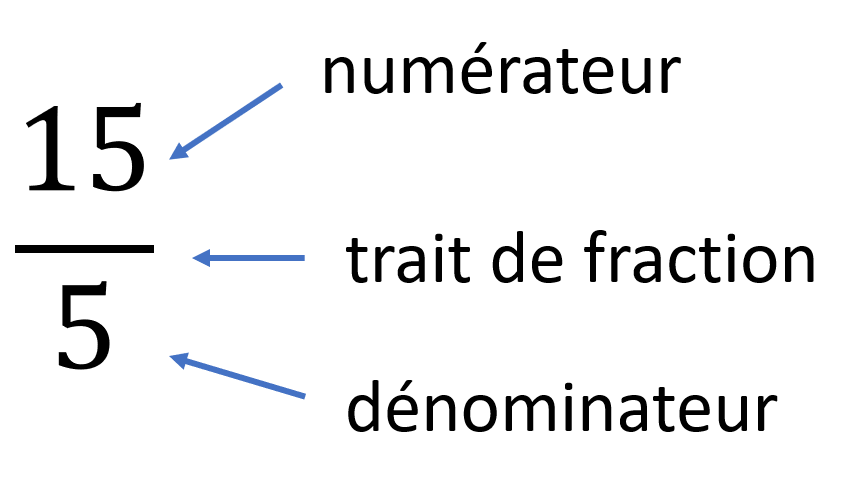
\includegraphics[scale=0.4]{img/frac2}
	\end{center}
\end{myex}

\begin{mydef}
	\begin{itemize}
		\item Une \kw{fraction décimale}, est une fraction où le dénominateur est un multiple de 10.		
		
		\item Toute fraction décimale peut s'écrire sous la forme d'un nombre décimal. C'est son \kw{écriture décimale}.
	\end{itemize}	
	
\end{mydef}


\begin{myexs}
	\begin{itemize}
		\item $\dfrac{145}{10}$ est une fraction décimale, son écriture décimale est \num{14.5}.
		\item $\dfrac{72}{100}$ est une fraction décimale, son écriture décimale est \num{0.72}.
		\item $\dfrac{9}{1000}$ est une fraction décimale, son écriture décimale est \num{0.009}.
	\end{itemize}
\end{myexs}


%
\section{Nombres et classement}
%
\begin{myact}{2 Classement}
	Activité 3 page 13
\end{myact}

\begin{myactrep}{2 Classement}
	\begin{enumerate}
		\item Le colis le plus lourd est celui qui a une masse de \num{15.3} kg et \num{13.999} kg pour le plus léger.
		\item On a donc :
		
		\num{13.999} < \num{14.15} < \num{14.509} < \num{14.575} < \num{14.59} <  \num{14.805} < \num{15.29} < \num{15.3}
	\end{enumerate}
\end{myactrep}

\begin{mydefs}
	\begin{itemize}
		\item \kw{Comparer} des nombres, c'est dire si un est plus petit ou plus grand que l'autre ou s'ils sont égaux.
		
		\item Ranger des nombres du plus petit au plus grand, c'est les classer par \kw{ordre croissant}.
		
		\item Ranger des nombres du plus grand au plus petit, c'est les classer par \kw{ordre décroissant}.
		
		\item \kw{Encadrer} un nombre, c'est trouver un nombre plus petit \textbf{et} un nombre plus grand que ce nombre.
		
		\item \kw{Intercaler} un nombre entre deux autres, c'est un nombre compris entre ces deux nombres.
	\end{itemize}
\end{mydefs}

\begin{myexs}
	\begin{itemize}
		\item 42 < 128, \pause se lit <<42 est inférieur à (ou plus petit que) 128>>;\pause
		\item 1337 < 1024,\pause se lit <<\num{1337} est supérieur à (ou plus grand que) \num{1024}>>;\pause
		\item 2 < \num{3.2} < \num{6.4} < \num{25.6} : ces nombres sont rangés dans l'ordre \pause croissant;\pause
		\item 123 > \num{45.6} > \num{7.89} > \num{5} : ces nombres sont rangés dans l'ordre \pause décroissant;\pause
		\item Encadrement de 21 à l'unité près : \pause 20 < 21 < 22 ;\pause
		\item Encadrement de \num{21.987} au centième près : \pause \num{21.977} < \num{21.987} < \num{21.997} ;\pause
	\end{itemize}
\end{myexs}

\begin{myexos}
	\begin{itemize}
		\item \Exo{16}{18} : Intercaler des nombres;
		\item Exercices 17 et 18 page 18 : Comparer des nombres;
		\item \Exo{19}{18} : Ordre croissant
		\item \Exo{20}{18} : Ordre décroissant
		\item Exercices 23 et 24 page 18 : Encadrer des nombres;
		\item \Exo{25}{19} : Comparer des nombres;
		\item \Exo{26}{19} : Ordre croissant;
		\item \Exo{27}{19} : Ordre décroissant.
	\end{itemize}
\end{myexos}


\begin{myprop}
	Un point placé sur une droite graduée est repéré par un nombre, son \kw{abscisse}.
\end{myprop}

\begin{myex}
	\begin{center}
		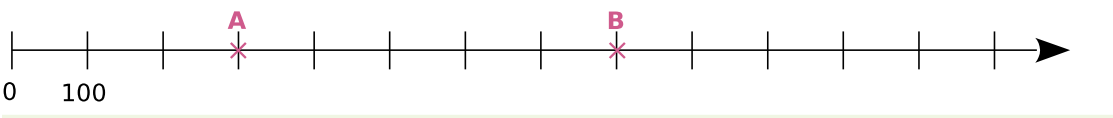
\includegraphics[scale=0.5]{img/axe}
	\end{center}

	\begin{itemize}
		\item L'abscisse du point A est :
		\item L'abscisse du point B est :
		\item L'abscisse du point C est : 500;
		\item L'abscisse du point D est \num{1100}.
	\end{itemize}
\end{myex}

\end{document}